\section{SAT Modelling}


\subsection{Problem Solving}


\begin{frame}{Idea: Problem Transformation}
\centering

\scalebox{0.6}{\begin{tikzpicture}
    \node (X) at (-3,1.5) {\foldedpaper{1}};
	\node at (-3,0.4) {Planning Problem};
    
	\draw[thick,line width=0.3mm,->] (-2,1.5) -- (-0.25,1.5);
	\node at (12,3) {};

    \node at (1,1) {\gear{10}{1.8}{2.4}{10}{2}{0.8}{0.2}};
    \node at (1.9,1.2) {\gear{10}{1.8}{2.4}{10}{2}{0.8}{0.2}};
    \draw (3,3) rectangle (0,0);
    \node at (1.5,2.5) {\only<2->{Transformer}\only<1>{Planner}};
    
    \draw[thick,line width=0.3mm,->] (3.25,1.5) -- (5,1.5);

	\node (X) at (6,1.5) {\foldedpaper{1}};
	\node at (6,0.4) {\only<4>{SAT problem}\only<2-3>{XYZ Problem}\only<1>{Plan}};
    
	\draw<3->[thick,line width=0.3mm,->] (7,1.5) -- (8.75,1.5);

    \node<3-> at (10,1) {\color{red}\gear{10}{1.8}{2.4}{10}{2}{0.8}{0.2}};
    \node<3-> at (10.9,1.2) {\color{red}\gear{10}{1.8}{2.4}{10}{2}{0.8}{0.2}};
    \draw<3-> (12,3) rectangle (9,0);
    \node<3-> at (10.5,2.5) {\only<3>{XYZ}\only<4->{SAT} Solver};
\end{tikzpicture}}
\end{frame}





\subsection{SAT}


\begin{frame}[fragile]{SAT}
 	\begin{definition}[SAT]
		Given a propositional formula $\mathcal F$, decide whether $\mathcal F$ has a satisfying valuation.
	\end{definition}
 	\begin{definition}<2->[CNF-SAT]
		Given a propositional formula $\mathcal F$ in conjunctive normal form, decide whether $\mathcal F$ has a satisfying valuation.
	\end{definition}
	\visible<3->{A valuation is an assignment of decision variables to $\{\top,\bot\}$.}\\[.25em]
	\visible<4->{CNF:}
	\[\visible<4->{\mathcal F = \bigwedge_{C \in \mathfrak C} \bigvee_{\ell \in C} \ell}\]
	\visible<4->{\vspace*{-1em}\begin{center}($\mathfrak{C}$ is the set of clauses; $C$ is a clause, a set of literals.)\end{center}}
	
\end{frame}






\subsection{SAT Solvers}


\begin{frame}[fragile]{SAT Solvers}
\begin{itemize}[<+->]
  \item SAT solvers are programs that determine whether a satisfying valuation exists and if so output it.
  \item A \textbf{lot} of research in recent years \\ (annual competitions since 2002).
  \item Usable OSes have \texttt{minisat} in their package manager.
  \item Standardised input format DIMACS:\\[0.3cm]
\begin{minipage}[t]{0.2\textwidth}\begin{verbatim}
p cnf 5 3
1 -5 4 0
-1 5 3 4 0
-3 -4 0
  \end{verbatim}\end{minipage} \quad \raisebox{-.75cm}{$\equiv$} \quad\ 
\begin{minipage}[t]{0.5\textwidth}%
CNF with 5 vars and 3 clauses:\\
$(v_1\vee\neg v_5\vee v_4)\ \wedge$\\
$(\neg v_1\vee v_5\vee v_3\vee v_4)\ \wedge$\\
$(\neg v_3\vee\neg v_4)$
\end{minipage} \quad
\end{itemize}
\end{frame}

\begin{frame}[fragile]{SAT Solvers -- IPASIR}
\begin{itemize}[<+->]
  \item Most SAT solvers support the IPASIR interface: \texttt{ipasir\_add}, \texttt{ipasir\_solve}, \texttt{ipasir\_val}
  \item Also allows for incremental solving via \texttt{ipasir\_assume} (if supported)
  \item Some SAT solvers have their own interface \texttt{kissat\_add}, \texttt{kissat\_solve}, \texttt{kissat\_val}\\[0.5cm]
  \item PySAT (includes some pre-defined encodings)
\end{itemize}
\end{frame}







\renewcommand*\VCShow{black}
\newcommand*\VCShoww{black}
\subsection{Modelling Example}




\begin{frame}{Colouring}
\begin{definition}
    Given a graph $G=(V,E)$ and a number $k$.\\
	Is there an assignment of $k$ colours to the vertices of $G$, such that all adjacent vertices have different colours?
\end{definition}
   
\begin{center}
     \only<1>{\renewcommand*\VCShow{black}}
     \only<1>{\renewcommand*\VCShoww{black}}
     \only<2->{\renewcommand*\VCShow{red}}
     \only<2->{\renewcommand*\VCShoww{blue}}
     \scalebox{0.75}{
 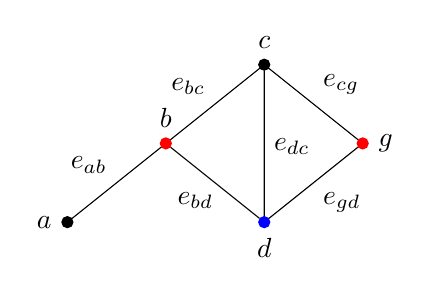
\begin{tikzpicture}[scale=1.0]
    \tikzstyle{N}=[draw,circle,fill=black,minimum size=4pt,inner sep=0pt]
    \draw (0,0) node (a) [N,label=left:$a$] {}
          to node[midway,auto] {$e_{ab}$} ++(1.25cm,1.0cm) node (b) [N,label=above:$b$,\VCShow] {}
          to node[midway,auto] {$e_{bc}$} ++(1.25cm,1.0cm) node (c) [N,label=above:$c$] {}
          to node[midway,auto] {$e_{cg}$} ++(1.25cm,-1.0cm) node (g) [N,label=right:$g$,\VCShow] {}
          to node[midway,auto] {$e_{gd}$} ++(-1.25cm,-1.0cm) node (d) [N,label=below:$d$,\VCShoww] {}
          to node[midway,right] {$e_{dc}$} (c)
          ;
   \draw (b) to node[midway,below] {$e_{bd}\hspace*{0.5cm}$} (d);
 \end{tikzpicture}
}

    \end{center}
\end{frame}






\begin{frame}{Colouring}
Variables for choosing the colour of each node
\[\mathtt{colour}_v^i \text{ where } v\in V \text{ and } i \in \{1,\dots,k\}\]
\pause
If a node has a colour, all adjacent nodes have a different colour
\[\mathtt{colour}_v^i \rightarrow \neg \mathtt{colour}_{w}^i \quad \quad \forall (v,w) \in E\]
\pause
\vspace{-0.5cm}
\[\neg \mathtt{colour}_v^i \vee \neg \mathtt{colour}_{w}^i \quad \quad \forall (v,w) \in E\]
\pause
Every node has a colour
\[\bigvee_{i=1}^k \mathtt{colour}_v^i \quad \quad \forall v \in V\]
\pause
Every node has at most one colour
\[\bigwedge_{i=1}^k \left[\mathtt{colour}_v^i \rightarrow \bigwedge_{j=1,i\neq j}^k \neg \mathtt{colour}_v^j \right] \quad \quad \forall v \in V\]
\end{frame}
	
